\documentclass{standalone}

\begin{document}

\section{Übung 2}

\subsection{DISCLAIMER - BITTE LESEN}
Aussagenlogik und Mengenlehre können manchmal extrem eklig sein, wenn man ein Zeichen oder ein Wort nur falsch abgelesen hat.
Hinterfragt (wie ihr es immer tun solltet) meine Lösungen auf alle Fälle und versucht sie nachzuvollziehen. 
Ich kann Fehler nicht ausschließen. Meldet euch gerne, wenn euch etwas aufgefallen ist, bevor einige Helden doch wieder nur die Lösungen auswendig lernen! (wobei Durchfallen dann verdient wäre\dots)

\subsection{Aufgabe 2.2}
"Among Us" in a nutshell\dots\\

Ansatz: Widersprüchliche Aussagen finden. Sobald zwei Personen sich widersprechen, ist bekannt, dass einer von ihnen Lügen muss. Die dritte verbleibende Person muss entsprechend die Wahrheit sagen, und ihre Aussage kann zur Entdeckung des Lügners beitragen.
\begin{itemize}
    \item A-B: Die beiden Aussagen hängen nicht zusammen, daher sind sie kongruent
    \item A-C: Die Aussagen widersprechen sich darin, ob A der Dieb ist oder nicht. A oder C müssen lügen.
    \item B-C: Die Aussagen widersprechen sich darin, ob B am Tatort war ("außer mir" heißt hier, dass B am Tatort war). B oder C müssen lügen.
\end{itemize}
Die jeweiligen Aussagen, ob jemand lügt oder nicht, müssen koexistieren können. Das bedeutet, dass wir die Schnittmenge beider Aussagen ermitteln. \\
A ODER C UND B ODER C, bzw $A \vee C \wedge B \vee C$ ist nur dann erfüllt, wenn der Lügner C ist. \\
Damit ist der Lügner C.

\subsection{Aufgabe 2.3}
Oben steht das Original (für Prüfung des Sinns weniger interessant), unten die nach Aufgabenstellung umgewandelte Version.
\begin{enumerate}[a)]
    \item \begin{gather}
        \forall n \notin \mathbb{P} \cup \{1\} \, \exists \, k \notin \{1,n\} : k \mid n \\
        \exists n \notin \mathbb{P} \cup \{1\} \, \forall \, k \notin \{1,n\} : k \mid n 
    \end{gather}
    Es existiert eine Zahl n, die keine Primzahl (oder 1) ist. Bei dieser gilt für alle k, die weder 1 noch die Zahl n sind, dass n durch k teilbar ist. \\
    Anders gesagt: es existiert eine Nicht-Primzahl (auch nicht 1), durch die alle Zahlen teilbar sind. \\
    Für $n=0$ funktioniert das, die Aussage ist wahr.

    \item \begin{gather}
        \forall x \in \mathbb{R} \, \forall \, y \in \mathbb{R} \setminus \{0\} : \frac{x}{y} \in \mathbb{R} \\
        \exists x \in \mathbb{R} \, \exists \, y \in \mathbb{R} \setminus \{0\} : \frac{x}{y} \in \mathbb{R}
    \end{gather}
    Es existiert eine reelle Zahl x, für die eine reelle Zahl y existiert (außer 0), sodass ihr Quotient in den reellen Zahlen liegt. \\
    Der Bruch zweier reeller Zahlen ist immer eine reelle Zahl (solange der Nenner $\neq 0$ ist). \\
    Die Aussage ist wahr.
    
    \item \begin{gather}
        \exists N \in \mathbb{N} \, \forall \, n \geq N : \frac{1}{n} \leq 0,001 \\
        \forall N \in \mathbb{N} \, \exists \, n \geq N : \frac{1}{n} \leq 0,001
    \end{gather}
    Für alle natürlichen Zahlen existiert eine Zahl n größer als sie selber, die invertiert $\leq 0,001$ ist. \\
    Die Zahl n ist nach oben unbeschränkt, und es muss nur ein n gewählt werden. \\
    Die Aussage ist wahr.

    \item \begin{gather}
        \exists n \in \mathbb{N} : \exists m \in \mathbb{N} : m+n > n^2 \\
        \forall n \in \mathbb{N} : \forall m \in \mathbb{N} : m+n > n^2
    \end{gather}
    Für alle natürlichen Zahlen n gilt, dass für alle natürlichen Zahlen m die Summe aus m und n $>n^2$ ist. \\
    Wähle m klein genug und n groß genug, dann geht die Aussage nicht mehr auf. \\
    Die Aussage ist falsch.
\end{enumerate}

\subsection{Aufgabe 2.4}
Strange community, aber in Ordnung\dots

Wir haben nur folgende zwei Gruppen im Dorf:
\begin{align}
    Gruppe\, A&,\, selber\, rasieren \\
    Gruppe\, B&,\, nur\, von\, Roberto\, rasieren\, lassen
\end{align}
Strikte Trennung, laut der Aufgabenstellung bedeutet, dass die Schnittmenge beider Gruppen leer ist, bzw.
$$ A \cap B = \emptyset $$

Roberto hat zwei Möglichkeiten, um seine Rasur zu bekommen:
\begin{itemize}
    \item Er geht zu einem anderen Barbier
    \item Er rasiert sich selbst
\end{itemize}
Wenn hergeleitet werden soll, dass Roberto nicht im Dorf wohnen kann, müssen wir beweisen, dass keine seiner Möglichkeiten ihn eindeutig einer der getrennten Gruppen im Dorf zuordnet.

Möglichkeit 1: Er geht zu einem anderen Barbier (Teilentscheidung $c$)
\begin{itemize}
    \item $c \notin A$, da er sich nicht selber rasiert
    \item $c \notin B$, da nicht Roberto (also er selbst), ihn rasiert
\end{itemize}
Keine Gruppe ist hier vertreten. Damit fällt Möglichkeit 1 aus.

Möglichkeit 2: Er rasiert sich selber (Teilentscheidung $c$)
\begin{itemize}
    \item $c \in A$, da er sich selber rasiert
    \item $c \in B$, da er sich nur von Roberto (keinem anderen) rasieren lässt
\end{itemize}
Beide Gruppen sind vertreten. Somit ist keine eindeutige Zuordnung (wie erforderlich) vorhanden, Möglichkeit 2 fällt aus.

\subsection{Aufgabe 2.5}

\begin{align}
    A&:=\{x \in \mathbb{R} \mid 5 > x > -2\} \\
    B&:=\{x \in \mathbb{R} \mid 1 > x\} \\
    C&:=\{x \in \mathbb{R} \mid -1 < x \leq 1\}
\end{align}

\begin{enumerate}[a)]
    \item $$ A \cap C = C $$
    \begin{itemize}
        \item Bestimmung der gemeinsamen Elemente von $A$ und $C$
        \item $C$ ist vollständig in $A$ enthalten, die Schnittmenge entspricht also $C$.
    \end{itemize}
    \begin{figure}[htpb]
        \centering
        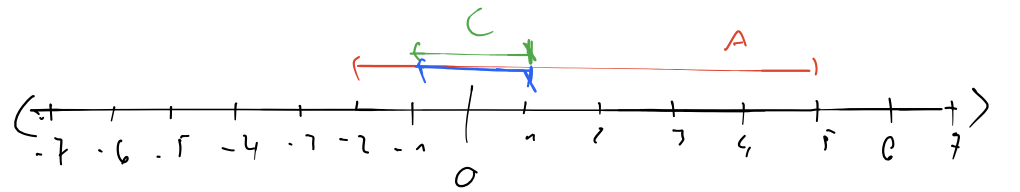
\includegraphics[width=10cm]{img/2_5_a}
    \end{figure}
    \FloatBarrier

    \item $$ B \setminus A = \{x \in \mathbb{R} \mid 2 \leq x\} $$
    \begin{itemize}
        \item Bestimmung der Menge $B$ ohne die Elemente von $A$
        \item $B$ enthält alle Elemente echt kleiner 1, $A$ nimmt aus B alle Elemente zwischen 1 und -2 (nicht einschließlich)
    \end{itemize}
    \begin{figure}[htpb]
        \centering
        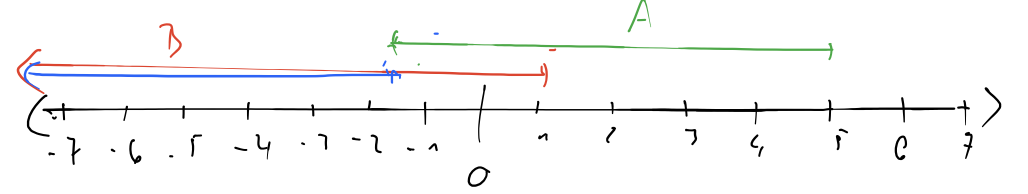
\includegraphics[width=10cm]{img/2_5_b}
    \end{figure}
    \FloatBarrier
    
    \item $$ (\mathbb{R} \setminus C) \cup B = \mathbb{R} \setminus \{1\} $$
    \begin{itemize}
        \item Zunächst die Elemente von $C$ aus allen reellen Zahlen entfernen, dann die Elemente von $B$ einfügen
        \item Da $B$ alle Elemente aus $C$ enthält, bis auf die eins ($\leq$ bei $C$ und $<$ bei $B$), fehlt aus dem Ergebnis nur die 1
    \end{itemize}
    \begin{figure}[htpb]
        \centering
        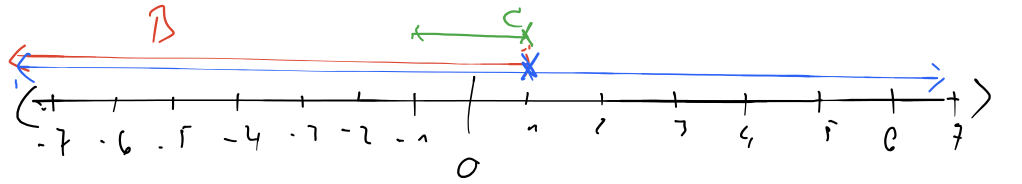
\includegraphics[width=10cm]{img/2_5_c}
    \end{figure}
    \FloatBarrier
\end{enumerate}

\subsection{Aufgabe 2.6}
Derselbe Spaß nochmal\dots

\begin{align}
    A&:=\{x \in \mathbb{R} \mid -3 < x < 4\} \\
    B&:=\{x \in \mathbb{R} \mid 2 \leq x\} \\
    C&:=\{x \in \mathbb{R} \mid -1 \leq x < 1\}
\end{align}

\begin{enumerate}[a)]
    \item $$ A \cup B = \{x \in \mathbb{R} \mid -3 < x\} $$
    \begin{itemize}
        \item Bestimmung der gesamten Elemente aus $A$ und $B$ zusammen
        \item $A$ geht bis -3 runter und überschneidet sich mit $B$, $B$ geht ins Unendliche hoch
    \end{itemize}
    \begin{figure}[htpb]
        \centering
        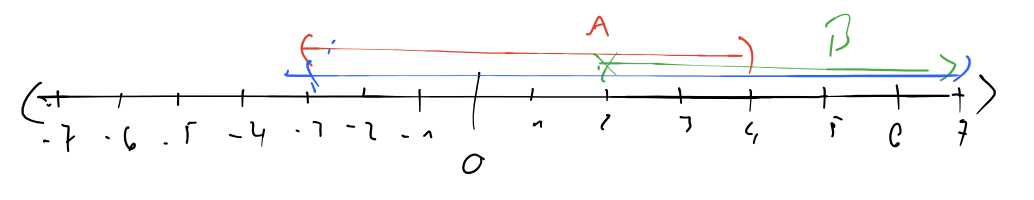
\includegraphics[width=10cm]{img/2_6_a}
    \end{figure}
    \FloatBarrier
    
    \item $$ C \cup (\mathbb{R} \setminus B) = \{x \in \mathbb{R} \mid 2 < x\} $$
    \begin{itemize}
        \item Bestimmung der gesamten Elemente aus $C$ und aller reellen Zahlen, abzüglich der Menge $B$
        \item $ \mathbb{R} \setminus B = \{x \in \mathbb{R} \mid 2 < x\} =: D $
        \item Alle Zahlen echt kleiner zwei werden $C$ hinzugefügt. Da $C \subset D$ ist, ist die Ergebnismenge $D$.
    \end{itemize}
    \begin{figure}[htpb]
        \centering
        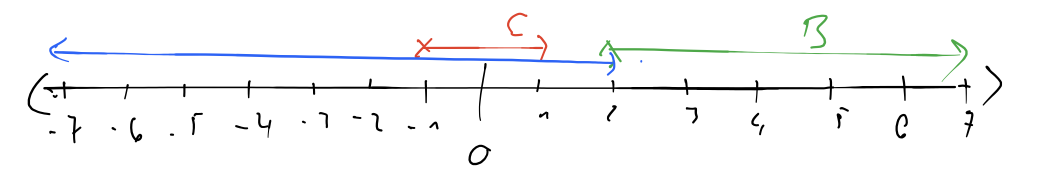
\includegraphics[width=10cm]{img/2_6_b}
    \end{figure}
    \FloatBarrier

    \item $$ (\mathbb{R} \cap B) \cup A = \{x \in \mathbb{R} \mid -3 < x\}$$
    \begin{itemize}
        \item Bestimmung der gesamten Elemente aus $A$ und den gemeinsamen Elementen aller reellen Zahlen und $B$
        \item Da $B \subset \mathbb{R}$ ist, ist $\mathbb{R} \cap B = B$
        \item Da $B \cup A = A \cup B$ ist, kann das Ergebnis einfach aus Teilaufgabe a) übernommen werden.
    \end{itemize}
    \begin{figure}[htpb]
        \centering
        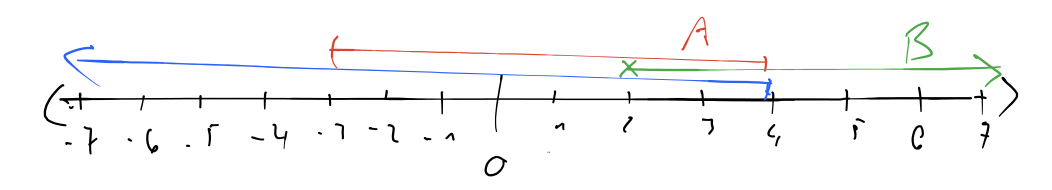
\includegraphics[width=10cm]{img/2_6_c}
    \end{figure}
    \FloatBarrier

    \item $$ ((A \cup B) \cap C) \setminus A = \emptyset$$
    \begin{itemize}
        \item $A \cup B = \{x \in \mathbb{R} \mid -3 < x\}$ wird aus a) übernommen
        \item $C \subset (A \cup B)$, damit ist $(A\cup B) \cap C = C$
        \item Da $C \subset A$ ist, ist $C\setminus A = \emptyset$
    \end{itemize}
    \begin{figure}[htpb]
        \centering
        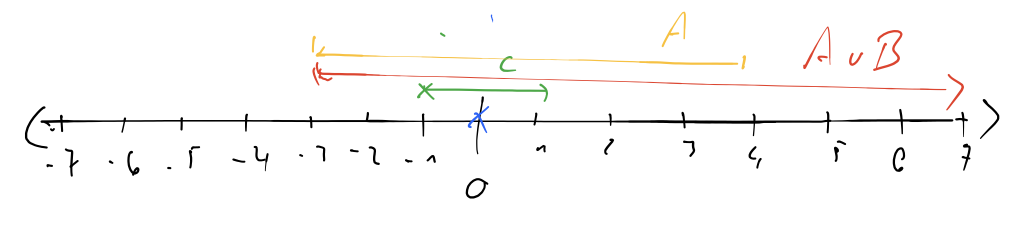
\includegraphics[width=10cm]{img/2_6_d}
    \end{figure}
    \FloatBarrier
\end{enumerate}

\subsection{Aufgabe 2.7}
Und ein drittes Mal, aber diesmal Quadrate\dots

\begin{align}
    A&:=\{x \in \mathbb{R} \mid -2 < x < 5\} \\
    B&:=\{x \in \mathbb{R} \mid 1 \geq x\} \\
    C&:=\{x \in \mathbb{R} \mid x^2 \leq 4\} \\
    D&:=\{x \in \mathbb{R} \mid x^2 > 1\}
\end{align}

\begin{enumerate}[a)]
    \item $$ A \cap B = \{x \in \mathbb{R} \mid -2 < x \leq 1\} $$
    \begin{itemize}
        \item Bestimmung der gemeinsamen Elemente von $A$ und $B$
        \item $A$ und $B$ überschneiden sich, $B$ liefert die Obergrenze der Elemente, da sie bis $-\infty$ weitergehen
    \end{itemize}
    \begin{figure}[htpb]
        \centering
        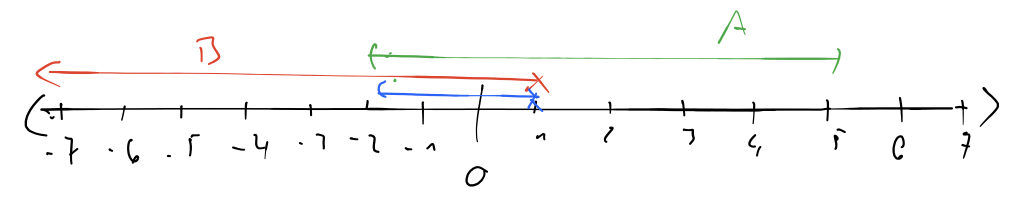
\includegraphics[width=10cm]{img/2_7_a}
    \end{figure}
    \FloatBarrier

    \item $$ A \cup D = \mathbb{R}$$
    \begin{itemize}
        \item Bestimmung aller Elemente aus $A$ und $D$ zusammen
        \item $D$ lässt sich umformen zu (siehe nächste Aufgabe) $D:= \mathbb{R} \setminus \{x \in \mathbb{R} \mid -1 \leq x \leq 1\}$
        \item $A$ füllt diese "Lücke" in den reellen Zahlen vollständig 
    \end{itemize}
    \begin{figure}[htpb]
        \centering
        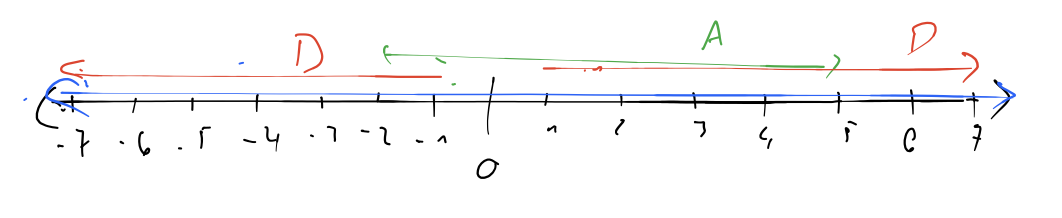
\includegraphics[width=10cm]{img/2_7_b}
    \end{figure}
    \FloatBarrier

    \item $$ B \setminus C = \{x \in \mathbb{R} \mid x < -2\}$$
    \begin{itemize}
        \item $C$ lässt sich durch Fallunterscheidung (bei geradem Exponenten fällt Vorzeichen weg) umschreiben zu $C = \{x \in \mathbb{R} \mid -2 \leq x \leq 2\}$
        \item $B$ und $C$ überschneiden sich, größtes Element von $C$ ist größer als größtes Element von $B$, aber $B$ läuft bis $-\infty$ weiter
        \item Außerdem $\leq$ (kleiner gleich) beachten, die -2 fällt aus der neuen Menge raus!
    \end{itemize}
    \begin{figure}[htpb]
        \centering
        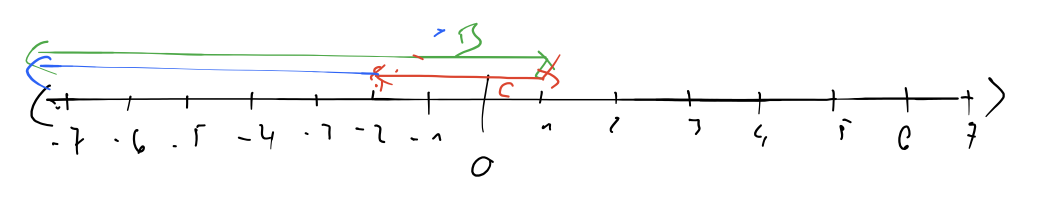
\includegraphics[width=10cm]{img/2_7_c}
    \end{figure}
    \FloatBarrier

    \item $$D \setminus (A \cap B) =  \{x \in \mathbb{R} \mid x \leq -2 \vee x > 1\}$$
    \begin{itemize}
        \item $A \cap B$ kann aus a) übernommen werden
        \item Wird erhalten zwei Bereiche: einen bis $+\infty$ über der Obergrenze von $A \cap B$ und umgekehrt
        \item Auf größer-kleiner-(gleich)-Zeichen achten!
    \end{itemize}
    \begin{figure}[htpb]
        \centering
        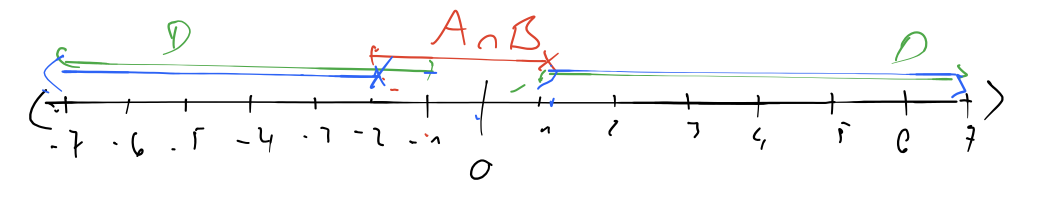
\includegraphics[width=10cm]{img/2_7_d}
    \end{figure}
    \FloatBarrier

    \FloatBarrier
    \item $$C \cap(A \cup B) = C$$
    \begin{itemize}
        \item $A \cup B = \{x \in \mathbb{R} \mid x < 5\}$, da $A$ und $B$ sich überschneiden und $B$ bis $-\infty$ weiterläuft
        \item $C$ ist vollständig in dieser Menge enthalten, also $C \subset (A \cup B)$
    \end{itemize}
    \begin{figure}[htpb]
        \centering
        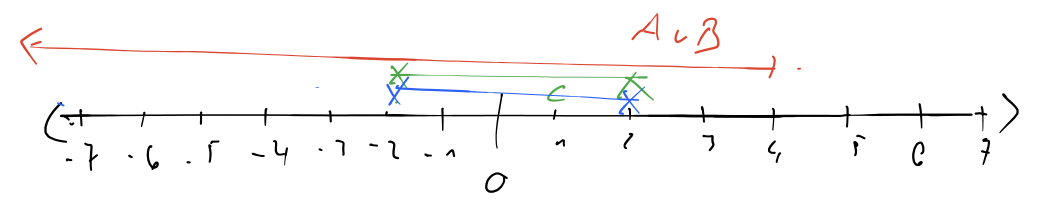
\includegraphics[width=10cm]{img/2_7_e}
    \end{figure}
    \FloatBarrier

    \item $$(\mathbb{R} \setminus (A \cap B))\cup (C \cap D) = \mathbb{R} \setminus \{x \in \mathbb{R} \mid -1 < x 1\}$$
    \begin{itemize}
        \item Eine Operation nach der anderen auflösen, dann bricht sich das schnell herunter
        \item $A \cap B$ kennen wir schon aus a)
        \item $\mathbb{R} \setminus (A \cap B)$ teilt sich wieder in zwei Mengen auf (quasi eine Lücke in den reellen Zahlen), mit 
        $\mathbb{R} \setminus (A \cap B) = \{x \in \mathbb{R} \mid x \leq\ -2 \vee x > 1\}$
        \item Für $C \cap D$ bildet $C$ die Obergrenze und $D$ die Untergrenze, es ergibt sich \\
        $C \cap D = \{x \in \mathbb{R} \mid x^2>1 \wedge x^2 \leq 4\}$, die Bedingungen sind mit dem UND-Operator verknüpft!
        \item Aus beiden Blöcken (links, rechts) wird zuletzt die Gesamtmenge gebildet
        \item Die einzigen Elemente aus $\mathbb{R}$, die in keiner beider Mengen vorliegen, sind \\
        $\{x \in \mathbb{R} \mid \ -1 < x < 1\}$
    \end{itemize}
    \begin{figure}[htpb]
        \centering
        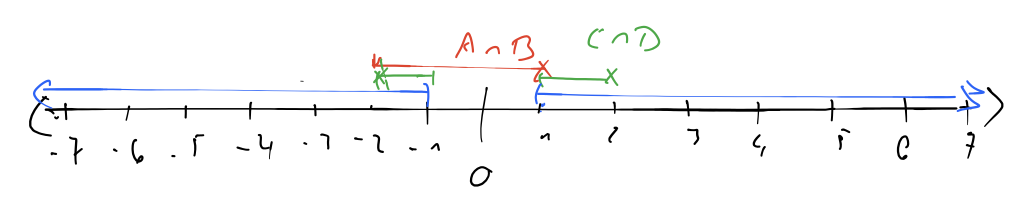
\includegraphics[width=10cm]{img/2_7_f}
    \end{figure}
    \FloatBarrier
\end{enumerate}

\subsection{Aufgabe 2.8}

\begin{align}
    M_1&:=\{1,2\} \\
    M_2&:=\{2,3\} \\
    M_3&:=\{X,y,3\} \\
    M_4&:=\{x,y,z\} \\
    M_5&:=\{2,4,6\}
\end{align}

\begin{enumerate}[a)]
    \item $M_1 \cap M_2 = \{2\}$
    \item $M_2 \cap M_3 = \{3\}$
    \item $M_3 \cap M_4 = \{3,X,x,y,z\}$
    \item $M_1 \cup M_2 \cup M_3 \cup M_4 \cup M_5 = \{1,2,3,4,6,X,x,y,z\} $
    \item $M_1 \cap M_2 \cap M_3 \cap M_4 \cap M_5 = \emptyset$
    \item $M_1 \times M_2 \times M_3 = \{(1,2),(1,3),(2,2),(2,3)\} \times M_3 = \\
    \{((1,2),X),((1,2),y),((1,2),3),((1,3),X),((1,3),y,((1,3),3),\\((2,2),X),((2,2)),y),((2,2),3),((2,3),X),((2,3),y),((2,3)),3)\}$
    \item Alle Paare disjunkter Mengen = $\{(M_1,M_3),(M_1,M_4),(M_2,M_4),(M_3,M_5),(M_4,M_5)\}$
    \item $M_1 \setminus M_2 = \{1\}$
    \item $M_3 \setminus M_4 = \{X,3\}$
\end{enumerate}



\end{document}
